\chapter{Related Work}
\label{chap:lit}

%This dissertation lies at the intersection of several fields including language testing, second language acquisition (SLA), intelligent computer-assisted language learning (ICALL), corpus linguistics and natural language processing (NLP). My work here is much indebted to related research in these areas, and in this chapter I summarize some of the most relevant studies.
This dissertation lies at the intersection of several fields including second language acquisition (SLA), intelligent computer-assisted language learning (ICALL), and natural language processing (NLP). My work here is much indebted to related research in these areas. In Section~\ref{section:SLA-overview}, I give a brief overview of SLA theory from the past several decades and its implications for language teaching. In Section~\ref{section:ICALL-overview}, I present a brief history of CALL and \textit{I}CALL, followed by a look at several influential ICALL projects. In Section~\ref{section:NLP-considerations}, I discuss the tools and techniques in NLP that I believe are suited for task-based, meaning-focused ICALL.


%I begin in Section~\ref{section:ICALLinterp} with a discussion of the importance of transparency and interpretability in ICALL and language testing. In  Section~\ref{section:ICALLoverview}, I examine approaches to ICALL that relate to and inform this dissertation. In Section~\ref{section:learnerCorpora}, I summarize research involving the collection, annotation or content analysis of task-based learner corpora. A brief overview of the NLP tools and methods used in my work is given in Section~\ref{section:NLP}.

%\section{On interpretability for learner applications}
%\label{section:ICALLinterp}
%
%(See also Section~\ref{section:imageProcessing}; this should address the use of sentence encoders like BERT and their use in conjunction with image recognition technology).
%
%This work would be remiss without discussing the role of machine learning (ML) in current NLP, given that such technologies are largely absent from this dissertation. Recent years have seen the rapid development of ML technologies like neural networks and deep learning. \lk{What is ML good at? citations!} These technologies have been widely implemented in areas like NLP and computer vision, often with impressive gains in performance. They can also lead to reductions in the amount of human expertise needed to automate tasks like syntactic labeling, voice recognition and synthesis, and object and facial recognition. \lk{cite stuff} Naturally, this also means significant reductions in the cost of such systems. A major drawback with many such ML technologies, however is the loss of interpretability. For example, \textit{word embeddings} (such as Word2Vec) \lk{cite} are ML based NLP tools suitable for many tasks involving the processing of linguistic meaning or structures. Word2Vec essentially ``learns'' an approximation of the meanings and grammatical usage of words by observing them in context. Instead of relying on expert annotation of features like part-of-speech, sentence structure and morphology to train a model, the system needs only large amounts of raw text. From this text, it observes large numbers of features, such as the average distance between instances of \textit{Word A} and \textit{Word B}. It reduces these raw features to a (still quite large) number of abstract features, or ``latent variables'', which form a vector of numeric values; this vector then serves as a representation of a word's ``meaning''. In a classic example, if one takes the vector for ``queen'', subtracts the vector for ``female'' and adds the vector for ``male'', the resulting vector is roughly equivalent to that of ``king''.
%
%\lk{this is all very cf Brian Riordan's alumni talk... similar sources would be ideal}
%For many applications, the capabilities and cost reduction of ML make it an attractive and suitable choice; this is certainly the case with many NLP tasks. The use of ML tools with learner language is problematic on at least two fronts, however. First, such tools are typically designed for and trained on well-formed, native-like text (or speech). As mentioned, these tools generally do not rely on annotation in their training data; instead, they make up for this lack of expertise by the sheer volume of training data they consume. Including real learner data on the scale required by ML tools would be impractical if not impossible for most researchers. As a result of ML tools' training on mostly native-like data, they are ill-equipped for processing the variability and ambiguity of learner language. For example, native English trained NLP tools expect regular sentence punctuation; text from a beginning English learner lacking in punctuation could therefore be misconstrued as having longer sentences and thus higher proficiency \cite{MeurersDickinson2017}. Second, and perhaps more importantly, tools that rely heavily on ML are inherently less interpretable than ``classical'' NLP tools. Because classical NLP tools are trained on expert annotation, their output is generally determined by the kinds of features that are annotated in the training corpus. This means linguistic researchers can design NLP tools and pipelines that produce output precisely suited for their research questions, so long as they have the resources to produce adequate training corpora. This is not the case with ML based tools, however. Due to their reliance on abstract features and latent variables, these newer tools are largely ``black box'' technologies; raw data goes in and processed data comes out, but even the architect of such a system cannot explain exactly how or why the analysis was produced. In a language learning application, this is problematic because it means the development of a pedagogically sound feedback system for the learner is not possible; the features underlying the analysis are not accessible or interpretable. The outcomes of language testing can have a tremendous impact on a test taker's future, and in such a high stakes application, the lack of interpretability can be even more problematic. Arguably, it is far better for all stakeholders if a language test can deliver not only a score, but also a rationale for that score, such as which kinds of errors a test taker makes and in what contexts. This need for interpretable features was one of a few major factors in the decision to choose classical NLP over newer ML tools in this dissertation, and most of the related studies discussed here take similar approaches.


%\section{Image processing}
%\label{section:imageProcessing}
%This should probably include discussion of ML approaches at image ``encoding/decoding'' and their use in tandem with sentence encoders (BERT, etc.). Ask Ben S. for reading suggestions?
%
%We want to touch on image processing / automatic captioning / use of semantic primatives, etc. -- linguistic annotation of images. NOT a deep discussion, but we need to acknowledge that there are other fields working on the relations between images and text, and give an idea of what some approaches are and how they work, and how they might relate to my work and the work discussed in my lit review.

\section{SLA \& Teaching Methodologies}
\label{section:SLA-overview}

SLA, the science of how humans learn a second language (L2), is largely concerned with the development of \textit{interlanguage}, the internal state of the learner's L2. As such, SLA research investigates the factors impacting L2 acquisition, such as the degree to which first language (L1) knowledge \textit{transfers} to the L2, the learner's \textit{access} to the brain's structures enabling L1 acquisition (the \textit{Language Acquisition Device}), the role of a \textit{critical period} for language acquisition, and the (un)predictability of the sequence in which L2 features are acquired. Naturally, the research and debates that take place in SLA  percolate into L2 teaching methodology and learner curricula.

With the emergence of modern linguistics in the
%late 1950s (\citealp[cf.][]{chomsky1957syntactic,chomsky1959behavior}), 
20th century, traditions in L2 teaching came under scrutiny by SLA researchers. The historically-dominant Grammar Translation Method (GTM), which \citet{richards2002longman} define as ``a method of foreign or second language teaching which makes use of translation and grammar study as the main teaching and learning activities,'' was primed for such critique. \citet{brown2000principles} refers to GTM as ``theoryless,'' arguing that the method ``does virtually nothing to enhance a student's communicative ability in the language.'' Instead, he suggests, GTM endures in many classrooms because it requires little of the instructor and tests are easy to construct and score.

The Audiolingual Method (ALM) emerged in the middle of the 20th century, as ``a rejection of its classical predecessor, the Grammar Translation Method, by diminishing if not obliterating the need for metacognitive focus on the forms of language'' \cite{brown2000principles}. As the name suggests, this method focuses on listening and speaking, with classrooms centered on listen-and-repeat drills entirely in the L2. ALM eventually fell out of favor among SLA professionals because it lacks both attention to grammar and realistic communication. Nonetheless, ALM exercises are still common in L2 classrooms around the world.

In the 1980s, the linguist Stephen Krashen's \textit{Input Hypothesis} of SLA and its pedagogical counterpart, the \textit{Natural Method}, rose to the forefront \cite{krashen1984,krashen1985}. Krashen suggested that learners really only need \textit{comprehensible input} in order to acquire an L2; given enough exposure, L2 speech will emerge. Crucially, L2 input should be only slightly beyond the learner's current interlanguage, a level that Krashen refers to as \textit{i+1}. Krashen assumes a difference between language \textit{learning} and language \textit{acquisition}, a distinction that not all linguists agree on (\citealp[cf.][]{white1987against}).

Krashen's theories of SLA were popular but also disputed, in large part for being untestable and inadequately-defined (e.g., \textit{i+1}), and for not distinguishing the processes of L1 and L2 acquisition. Nonetheless, Krashen's ideas have remained influential in L2 learning contexts and the shift from \textit{teacher-centered} and \textit{form-focused} to \textit{student-centered} and \textit{content-focused} methodologies. \textit{Extensive reading}, for example, is common in L2 learning contexts and involves students reading large amounts of material at a comprehensible level, without accompanying instruction, exercises, or comprehension tests \cite{mason1997extensive,day1998extensive}. Moreover, SLA research has shown this practice to be effective at improving learners' L2 abilities \cite{renandya2007power,nakanishi2015meta}. Likewise, in \textit{extensive listening}, learners listen to comprehensible L2 speech, with an emphasis on consuming large amounts of material unburdened by the need to look up vocabulary items or perform comprehension exercises \cite{renandya2011teacher}. Studies have also shown extensive listening to be effective for L2 learners \cite{zhang2005investigation,zeng2018self}. With the explosion of podcasts, mobile phone apps, and digital platforms for sharing audio and video, extensive listening has grown in popularity both inside and outside the classroom \cite{vo2013developing,gonulal2020improving}.

As Krashen's theories relied on the \textit{interlanguage} of individual L2 learners, SLA research of the era came to emphasize the role of individual differences in L2 acquisition. Differences like motivation, age, personality, and learning styles came to be seen as important factors, and thus as \citet{brown2000principles} explained, the field came to see the methods of the past as ``too narrow and too constrictive to apply to a wide range of learners in an enormous number of situational contexts.'' Instead, pedagogical trends shifted away from methods and toward ``approaches'' that are founded on principles but adaptable to different contexts and learners.

Chief among these approaches are \textit{Communicative Language Teaching} (CLT) and \textit{Task-Based Language Teaching} (TBLT), both of which are widely applied in some form in L2 classrooms today. CLT and TBLT have much in common, and indeed TBLT is sometimes considered a subset of CLT. Both approaches emphasize the importance of ``authentic'' materials and situations, learner interaction, and the use of the L2 to negotiate meaning and exchange information \cite{littlewood1981communicative,canale2014communicative,long2016defense}. \citet{ellis2009task} defines a \textit{task} as a ``pedagogic activity where the learners are provided with L2 data in some form and required to perform some operation on or with it, the purpose of which is to arrive at an explicit understanding of some linguistic property or properties of the target language.'' While the principles of CLT and TBLT are widely accepted today, there are disagreements about the effectiveness of these approaches in large classroom settings where their application is difficult, and about the role of the L2 instructor \cite{rahman2018exploring}. There are also disagreements about the extent to which CLT and TBLT can replace more traditional instruction. The strictest positions on CLT and TBLT largely reject traditional, teacher-centered instruction (\citealp[cf.][]{skehan1998cognitive,long1985role}), while others support a ``hybrid'' approach; \citet{ellis2009task} argues that traditional structural teaching is complementary to TBLT, with tasks reinforcing classroom instruction.  A meta-analysis of 52 studies found that TBLT programs in L2 are both effective at improving learner outcomes and positively viewed by learners \cite{bryfonski2019tblt}.

A major drawback to TBLT and CLT is the amount of time and effort required of instructors in finding and preparing authentic materials and designing communicative tasks. Studies on impressions of TBLT found that instructors often cite the lack of appropriate teaching materials and the cost of producing their own as one of the biggest problems with the approach \cite{zheng2014task}; the difficulty of implementing student-centered TBLT in large classrooms is another \cite{harris2018responding}. In the following sections, I look at past and present ICALL projects and the potential for ICALL to support the work of task-based and communicative teaching.


%Today, many of the pedagogical springs and rivers of the last few decades are appropriately captured in the term Communicative Language Teaching (CLT), now a catch phrase for language teachers. CLT, to be discussed further in Chapter 8, is an eclectic blend of the contributions of previous methods into the best of what a teacher can provide in authentic uses of the second language in the classroom. Indeed, the single greatest challenge in the profession is to move significantly beyond the teaching of rules, patterns, definitions, and other knowledge "about" language to the point that we are teaching our students to communicate genuinely, spontaneously, and meaningfully in the second language. \cite{brown2000principles}

%This historical evolution can be interpreted partly as a struggle to offer learners an increasingly
%inclusive experience of language. Thus while grammar-translation was organised largely around
%texts of a literary nature, audiolingualism focused on ensuring systematic coverage of the structural
%repertoire of a language. Despite its thoroughness, a significant part of the reaction against audiolingualism
%could in turn be seen as a response to the impoverished picture of language that the approach
%offered. Structures were essentially isolated from typical discourse environments, and contextualised
%mainly within stimulus-response-feedback sequences. \cite{brown2000principles}

%Communicative methods \& TBLT; where does SLA point to the need for content-focused, task-based systems like mine?
%
%DEFINE TASK \& TBLT
%
%``an activity that is communicative at some level, but whose purpose, overt or covert, is to practice specific linguistic items.''
%\cite{long2016defense}
%
%``A pedagogic activity where the learners are provided with L2 data in some form and required to perform some operation on or with it, the purpose of which is to arrive at an explicit understanding of some linguistic property or properties of the target language.''
%``Task-based teaching need not be seen as an alternative to more traditional, form focused approaches but can be used alongside them � (Long and Skehan view traditional structural teaching as theoretically indefensible while I see it as complementary to TBLT).''
%\cite{ellis2009task}



\section{ICALL}
\label{section:ICALL-overview}

%Here I need a brief overview of CALL and ICALL, the transition from CALL to ICALL, and the need for ICALL to work with SLA...

Given the prominence of task-based and communicative approaches to L2 teaching, coupled with the difficulties facing instructors in preparing tasks tailored for their students, and given the current availability of powerful NLP tools, I believe the time is right for ICALL to fill the void. To this end, I began this dissertation project as an experiment in bootstrapping NLP tools, native speaker data, and learner data to achieve meaning-based ICALL. I do not attempt a full-fledged ICALL system, but I explore mechanisms for performing the core content analysis that could be implemented in a setting like an ICALL game (see Chapters~\ref{chap:pilot} and~\ref{chap:optimization}). I see this work as a push toward CLT-oriented, relatively low-cost, extendable ICALL with an emphasis on content over form. In the next section, I present a brief summary of the early history of CALL and ICALL, intended as context for the sections that follow, where I examine a number of more recent ICALL projects that inspired my own work.

%... ICALL projects that share one or more aspects of my approach, namely the use of existing NLP tools, the processing of free user input (as opposed to menu-based or fill-in-the-blank input), and the use of crowdsourced response models.


\subsection{From CALL to Early ICALL}
\label{section:CALL-ICALL}
The history of ``\textit{un}intelligent'' CALL can be traced to the early 1960s, when the audiolingual method (ALM) was widespread in L2 teaching. ALM's emphasis on drills and repetition was a good match for the rudimentary technology of the time \cite{heift:schulze:07}. CALL systems at this time were mainframe systems implemented at universities and accessed by students at terminals in language labs. Examples of such systems are PLATO (Programmed Logic for Automated Teaching Operations), begun in 1960 at the University of Illinois and TICCIT (Time-shared Interactive Computer Controlled Information Television) at the University of Texas and Brigham Young University. These were intended as scalable subscription services, available to other universities and institutions remotely via telephone lines, but their adoption was severely hindered by the high cost of long-distance connections \cite{levy1997computer}. 

This problem was eliminated with the advent of microcomputers, and CALL systems proliferated throughout the 1980s. These systems nonetheless focused on drills for reading, grammar, and vocabulary, with an emphasis on accuracy, lagging behind the student-centered trends in L2 teaching methodology \cite{kannan2018new}. CALL in this period still faced practical technological obstacles; the landscape of diverse operating systems meant that most CALL projects were not accessible to large numbers of users \cite{davies2013historical}.

The arrival of sound cards in the late 1980s enabled the integration of listening and speaking activities in CALL applications. The consolidation of operating systems, steady increases in computing power, and the expanding market for personal computers in the late 1980s and early 1990s helped usher in the shift toward \textit{intelligent} CALL, although the term \textit{ICALL} is attested as early as 1978 \cite{levy1997computer,thomas2013role}. Stemming from this period, as noted by \citet{ai2017providing}, ``the conventional understanding of the notion of `intelligence' in ICALL research leans more toward technology than toward language learning.'' Indeed, much ICALL literature of the 1990s is marked by a giddiness about implementing state-of-the-art technology and only a passing interest in SLA; as one fictional character of the era put it, ``Your scientists were so preoccupied with whether or not they could, they didn't stop to think if they should'' \cite{jurassic1993}. Or less glibly, early ICALL projects were designed more around the capabilities of the technology than principled approaches to L2 teaching and learning.

\textit{Rosetta Stone}, first launched in 1992, was a prime example of this technology-driven approach to CALL. The core of these early versions were drills in which users view an image and click a corresponding sentences, or vice versa. The program was criticized by SLA researchers and language teaching professionals of the time, with complaints highlighting its lack of discourse, lack of culturally appropriate images and content, emphasis on repetitive drills, and limited range of activities (\citealp[cf.][]{lampugnani1998rosetta,kaiser1997rosetta}).

The 1990s saw the consolidation of ICALL around research venues like \textit{CALICO} and \textit{EuroCALL}. Much of the work in this period focused on using new methods in statistical language modeling to identify learner errors, but the decade also saw the first serious attempts to integrate outside research and apply empirical measures of L2 learning outcomes \cite{thomas2013role}.
As a result, ICALL systems began to emerge that were arguably more ``enlightened'' with regard to SLA and L2 teaching methodology. In the following sections, I shift my focus to a number of ICALL projects that appeared from the mid-1990s through the early 2010s and describe how these systems helped shape my own approach.

\subsection{Herr Kommissar}
\label{section:herr-kommissar}


\textit{Herr Kommissar} \citep{desmedt1991herr,desmedt:95} is an ICALL system for German learners that includes rather robust content analysis and sentence generation and represented significant progress in the integration of communicative and task-based learning in ICALL. The system is styled as a game in which the user plays the role of an American detective traveling through the German countryside who is called upon by local police to help solve murders. To progress through the game and solve mysteries, the user must interview witnesses and interrogate suspects. The user is assisted throughout these dialogs by a local detective. The local detective is effectively the system's feedback agent, providing corrections and recasts of the user's German as well as hints regarding content. In this way, Herr Kommissar set a high bar by cleverly disguising language instruction as realistic communication to create an immersive learning experience and was generally well-received by learners and instructors \cite{harroff1993herr}.

This ICALL system was ambitious and in many ways was ahead of its time---the sentence parsing, sentence generation, language modeling and computing power of the 1990s were not equipped to handle complex discourse. To overcome technical limitations, ``behind the scenes'' the system relied on a great deal of hand-built tools, custom decision trees, string matching, and template-based responses that were tailored to the scenario at hand. When users presented off-target or incomprehensible input, the system relied on the assistant detective to redirect conversations, keeping the game ``on the rails'' and maintaining the illusion of authentic conversation. Naturally, these scenario-dependent pipelines were not easily adaptable to new contexts. Nonetheless, Herr Kommissar was a step forward for task-based ICALL and a major inspiration for the work presented throughout this dissertation. In a practical sense, my work started with the goal of enabling an ICALL game like Herr Kommissar using a more versatile approach to handling user input and less of the hidden, story-specific processing. 

\subsection{C-Rater and Related ETS Projects}
\label{section:c-rater}

The development of c-rater (\textit{concept} rater; \citealp{leacock:chodorow:03,sukkarieh2008leveraging}) at Educational Testing Services (ETS) marked a significant step forward in the analysis of free-input text. C-rater began as a system for scoring short answer responses to reading comprehension tests in the \textit{Test of English as a Foreign Language} (TOEFL) and was later made available on the internet for instructors to develop tests and exercises. While c-rater is primarily an assessment tool, it overlaps with research in ICALL and has had a lasting influence on the field \cite{burrows2015eras}.

The system is essentially a paraphrase recognizer. Each question must have a discrete range of correct answers, and a model answer is supplied by an expert. The role of the system is to use a partial sentence parser \citep{abney1996partial} to identify verbs and their arguments in this expert answer, and apply a lemmatizer to represent these key words in their uninflected forms. The system then handles a user response in the same fashion and attempts to map the resulting verbs and arguments to the expert answer. This representation of sentences as verbs and their arguments allows c-rater to match concepts across variations in syntax; my own work on content analysis borrows from this approach (see Section~\ref{sec:semantic-form}). The researchers explored using simple bag-of-words representations of sentences, but found that this underperforms their concept representation.

To overcome variations in lexical items and their phrasing, c-rater uses a word similarity matrix, trained on a corpus of over 300 million words to expand the query; this method groups similar words according to the contexts in which they appear \cite{lin1998information}. Responses are marked as either complete, partially complete, or incomplete. The researchers reported average agreement between c-rater and human raters at 84\% with a kappa of 0.74. 

The work on c-rater led to later research at ETS on evaluating responses to visual prompts that is more directly applicable to the kinds of contexts I pursue in this dissertation. \citet{somasundaran:chodorow:14} present work in which they automatically score L2 learner responses to a picture description task (PDT) on a four-point scale, using much of the same processing as c-rater. A common concern for any content evaluation system is the handling of the wide variety of ways a concept can be expressed. Here, the researchers constrain the range of input by providing users with two lexical items and instructing them to use those words in their responses. Like c-rater, this system relies on expert response models, but in this case a more robust model is used. The researchers call this a \textit{reference text corpus}, where the expert lists all items and events in the image and thoroughly describes any events and relationships depicted. The researchers reported a kappa of 0.63 for the system's agreement with human scores, versus 0.83 for human-human agreement.

In my own work here, which also uses PDTs, I considered providing users lexical items, but ultimately did not directly pursue it. Instead, I focused on constraining the responses by limiting the amount of information in the image prompts, and I relied on crowdsourcing a corpus of native speaker responses instead of a single expert's exhaustive description (Sections~\ref{sec:pdt} and~\ref{sec:participants}).

%\cite{somasundaran:ea:15} %% 6-image spoken image narration.


\subsection{Robo-Sensei}
\label{section:robo-sensei}
Robo-Sensei is an ICALL system for English-speaking learners of Japanese that was developed in conjunction with a textbook series and used in classrooms starting in 2005 \cite{nagata2009robo}. This system bears much in common with the methods used in c-rater: its main analysis is conducted with a morphological parser (cf. c-rater's \textit{lemmatizer}) and a syntactic parser, which transform student input into a representation of sentence elements like verbs and their arguments. However, Robo-sensei relies on expert response models that are manually created in this same abstracted representation. Rather than using an automatically-generated lexical similarity matrix, the expert manually provides a list of synonyms for each lexical item in the expert representation, and the system expands on the representation by exhaustively replacing all lexical items with these synonyms.

The system's main exercise centers on ``communicative contexts,'' presented to the user in the L1 (English) in the second person, e.g., ``Your teacher asked how your weekend was.'' These contexts also provide the content for the user's response, e.g., ``You had a big party for your father's birthday and had to wash many dishes afterward.'' The user must then provide a short answer in the L2 (Japanese) consisting of one or more sentences. Like the provided lexical items in \citet{somasundaran:chodorow:14}, this provided information is a strategy for constraining the range of acceptable responses. The user response is processed into the system's representation and compared against the elements in the expanded expert model; the results of this comparison are passed to Robo-sensei's feedback module, which uses a relatively complex system of templates to generate form-focused feedback. 

The system's pipeline of normalizing word forms and parsing sentences into subcomponents representing meaning influenced my approach, but I diverged from many of the strategic choices made in Robo-Sensei. The use of the L1, while understandable from a practical point of view, more closely resembles the Grammar Translation Method than I wish for my own work. 

\subsection{TAGARELA}
\label{section:tagarela}
One relatively well-documented and SLA-informed ICALL system is TAGARELA (\textit{Teaching Aid for Grammatical Awareness, Recognition and Enhancement of Linguistic Abilities}), an application for adult learners of Portuguese \cite{amaral2007designing,amaral:meurers:user:07,Amaral.Meurers.Ziai-11}. TAGARELA was developed at The Ohio State University and used by beginning Portuguese learners enrolled there. It relies on a set of NLP modules implemented in a task-based, free input ICALL system. The system includes six different activity types: reading, listening, description, rephrasing, vocabulary and fill-in-the-blank. These different tasks require different types of textual learner input as well as different subsets of the NLP modules for input processing and the generation of feedback.

A crucial component to TAGARELA is its ``Unstructured Information Management Architecture (UIMA),'' which is effectively a collection of text relevant to the tasks that are enriched with multiple annotations relating to both form and meaning. For most tasks, this means TAGARELA relies on a small number of carefully chosen and annotated model responses. This \textit{UIMA} approach means TAGARELA can use a given model in different tasks by varying the NLP pipeline and the selecting the appropriate annotation layers. This approach is also its biggest obstacle, however: each new lesson in TAGARELA requires the careful, deliberate development and testing of expertly annotated model responses. In other words, the system must be ``told'' explicitly what to look for in a user response.

In fairness, TAGARELA was not designed to be a fully-fledged ICALL system ready for widespread use, but rather as an experiment and a data collection tool for ICALL researchers, and in this regard, it stands as a successful project and an important step toward handling meaning in ICALL with cleverly-implemented NLP. Prior to any system development, the TAGARELA team began their work with the creation of a ``taxonomy of expected errors,'' gleaned from an analysis of a corpus of written assignments from learners of Portuguese. The authors describe this development approach as ``data-driven rather than process-driven.'' This bucks a tendency among many ICALL developers to simply address the kinds of errors NLP tools can readily identify. 
%\lk{cite DuoLingo? etc.}
%What is needed instead is ICALL development informed by SLA research and by the kinds of challenges learners face, as borne out by real data.
%\lk{cite Ellis, Meurers}
The errors annotated in the Portuguese learner data and handled by TAGARELA cover both form and meaning, with error types consisting of, for example, \textit{spelling}, \textit{agreement} and \textit{word choice}.
My work was inspired by TAGARELA's data-driven approach, and especially by its prioritization of the handling of errors related to meaning. Moreover, TAGARELA demonstrated for ICALL the successful use of ordinary and interpretable NLP tools---primarily a tokenizer, part of speech tagger and syntactic parser.

\subsection{E-Tutor}
\label{section:e-tutor}

E-Tutor is an ICALL workbook-style application for English-speaking L2 German learners designed to parallel a widely-used textbook series \cite{heift:01,heift2010,heift2018querying}. The program relies on English for instruction and scaffolding around the grammar and vocabulary lessons it presents. It includes activities with varying degrees of free-input. The simplest are grammar and vocabulary exercises that ask users to complete sentences or build their own using provided lexical items. More sophisticated exercises ask users to write their own sentences in response to reading comprehension questions.

Most of E-Tutor's exercises require a robust set of pre-stored answers provided by an expert. The system relies on string matching to evaluate user responses. To handle variations not covered in the expert set, E-Tutor passes unmatched user responses through what the researchers call its ``error sieve,'' a pipeline of modules that either apply variations (or corrections) to punctuation, spelling, or word order, or check for missing or extra words or ungrammatical constructions. When one of these modules results in a string match with the expert set, a form-focused feedback message is presented to the user.

An appealing feature of this system is its ability to expand its models over time by identifying learner responses that do not match an expert response but also do not trigger its error detection modules. My work does not reach the stage of development where such a strategy could be applied, but my reliance on crowdsourcing to compile models is partly inspired by E-Tutor's approach of using non-expert responses collected from users. In terms of methodology, E-Tutor could benefit from more authentic communicative tasks and content-focused feedback. With regard to its application of NLP, the system handles a considerable range of activities with its modular pipeline. However, E-Tutor uses the technology almost exclusively for error identification rather than attempting to address meaning. 




%For instance, the activity types in the E-Tutor (Heift, 2010b)
%allow for grammar practice as well as reading comprehension and/or cultural knowledge
%and also supports discovery learning in the form of exploration of learner language. For
%this, user submissions over five years were compiled and from those a common learner
%corpus was constructed that allows students to explore learner language according to
%various parameters. Thus, learners can examine interlanguage or task-specific phenomena
%and the benefits in this respect have been well documented (Granger, 2003a). Moreover, 
%these large data sets also allow language instructors and/or researchers to examine the
%design of language learning material in addition to a wide range of additional research
%topics (e.g., use of help options, interlanguage studies).
%Similarly, Robo-Sensei developed by Nagata (2009) for L2 learners of Japanese
%analyses student input for selected exercises, performs an itemization (separating tokens
%for later linguistic analysis) and a morphological analysis, and parses the sentential input
%syntactically using a context-free grammar. Finally, Tagarela (Amaral \& Meurers, 2011)
%an ICALL system for Portuguese is similar to the E-Tutor and RoboSensei, in that it uses
%the metaphor of an electronic textbook. The system provides practice with grammar and
%listening comprehension and students receive feedback on spelling, morphological,
%syntactic and semantic errors. These three systems are used in the regular L2 language
%classroom.




\subsection{Sasha dialog agent}
\citet{petersen:10} presented \textit{Sasha}, an ICALL system for simulating dialogs with L2 English learners in visual contexts. The system was designed specifically for eliciting questions about images; in these scenarios, the learner is instructed to ask Sasha questions about objects, relationships and events in the image prompt. Sasha serves as the interlocutor and asks for clarification, provides recasts, and responds to the user question with appropriate information in sentence form. The task is a kind of information gap task in which the user is presented with multiple images and must determine which of the images Sasha is viewing. These interactions are not sustained discourse, but rather unordered dyads that continue until the user is ready to identify the correct image.

The system uses standard NLP modules combined in a custom, rule-based pipeline to process user input. The modules generate a rich internal representation that includes spelling correction, part of speech tagging, word sense disambiguation, synonym set identification, and syntactic dependency parse information. To generate an appropriate response, Sasha relies on an expert-produced  list describing objects and relationships in the images. Sasha also uses a set of rules and templates for generating responses to various question types by filling templates with the appropriate content from the expert descriptions.

My work was partly inspired by Sasha's use of images to focus ``discussion'' and its use of dependency parse information and rules for extracting elements like subjects and objects in order to generate internal representations of meaning that abstract over specific forms, particularly in my pilot study (Section~\ref{sec:pilot-study}.)

\section{NLP for task-based ICALL}
\label{section:NLP-considerations}

What kinds of processing are necessary and useful for my ICALL needs?

Address interpretability;

auto image-captioning;

Dependencies;

tf-idf and distributional semantics;




%
%%%%%%%%%%%%%%%%%%%%%%%%%%%%%%%%%%%% BELOW: \cite{meurers:12} %%%%%%%%%%%%%%%%%%%%%%%%%%%%%%%%%%%%%%%%%%%%%%%%%%
%\bigskip
%NOTES:
%\bigskip
%
%for the wide range of language activities supporting significant well-formed
%or ill-formed variation of form, meaning, or task-appropriateness of learner responses, it is
%necessary to abstract away from the specific string entered by the learner to more general
%classes of properties by automatically analyzing the learner input using NLP algorithms and
%resources. 
%
%...
%
%Nagata, N. (2009). Robo-Sensei�s NLP-Based Error Detection and Feedback Generation.
%CALICO Journal 26(3), 562�579. URL http://purl.org/calico/nagata09.pdf.
%
%Nagata (2009, pp. 563f) provides a clear illustration of this with an exercise taken from her
%Japanese tutor ROBO-SENSEI in which the learner reads a short communicative context and
%is asked to produce a sentence in Japanese that is provided in English by the system. The
%learner response in this exercise is directly dependent on the input provided by the exercise
%(a direct response in the terminology of Bachman \& Palmer, 1996), so that a short, seven
%word sentence can be defined as target answer. Yet after considering possible well-formed
%lexical, orthographic, and word order variants, one already obtains 6048 correct sentences
%which could be entered by the learner. Considering incorrect options, even if one restricts
%ill-formed patterns to wrong particle and conjugation choices, one obtains almost a million
%sentences.
%
%...
%
%Complementing the analysis of form, for an ILTS to offer meaning-based, contextualized ac
%tivities
%it is important to provide an automatic analysis of meaning aspects, e.g., to determine
%whether the answer given by the learner for a reading comprehension question makes sense
%given the reading.
%
%%%%%%%%%%%%%%%%%%%%%%%%%%%%%%%%%%%% ABOVE: \cite{meurers:12} %%%%%%%%%%%%%%%%%%%%%%%%%%%%%%%%%%%%%%%%%%%%%%%%%%



%\section{Learner corpora}
%\label{section:learnerCorpora}
%Here I will discuss task-based learner corpora research that relates to my work. This includes discussions of task design, data collection, annotation schemes, and automatic processing. I focus in particular on the learner content analysis research conducted by two clusters of researchers: one primarily associated with The Ohio State University and consisting of Detmar Meurers and colleagues, and the other primarily associated with Educational Testing Services (ETS) and consisting of Martin Chodorow, Swapna Somasundaran and Joel Tetrault and colleagues. 
%
%Here are some papers I discussed briefly in my BEA 2018 paper:
%
%\cite{leacock:ea:14}
%
%\cite{kyle2015automatically}
%
%\cite{weigle2013english}
%
%\cite{amaral:meurers:user:07}
%
%\cite{Meurers.Dickinson-17}
%
%\cite{heift:schulze:07}
%
%\cite{somasundaran:ea:15}
%
%\cite{bailey:meurers:08}
%
%\cite{meurers2011evaluating}
%
%\cite{somasundaran:chodorow:14}
%
%\cite{cahill-et-al:14}
%
%\cite{ragheb:dickinson:14a}
%
%\cite{foster2009native}
%
%\cite{cho2013investigating}
%
%\cite{landis1977measurement}
%
%\cite{artstein:massimo:2008}
%
%\cite{tetreault-chodorow:2008:HJCL}
%
%\cite{tetreault:chodorow:08}
%
%\section{Language assessment}
%\label{section:languageAssessment}
%
%\section{NLP tools and methods}
%\label{section:NLP}
%
%\section{My previous work}
%\label{section:myPreviousWork}
%Here I will discuss the work I have previously done in this area, including the papers given in the subsections below.
%
%\subsection{2013}
%\cite{king:dickinson:13}
%
%\begin{figure}
%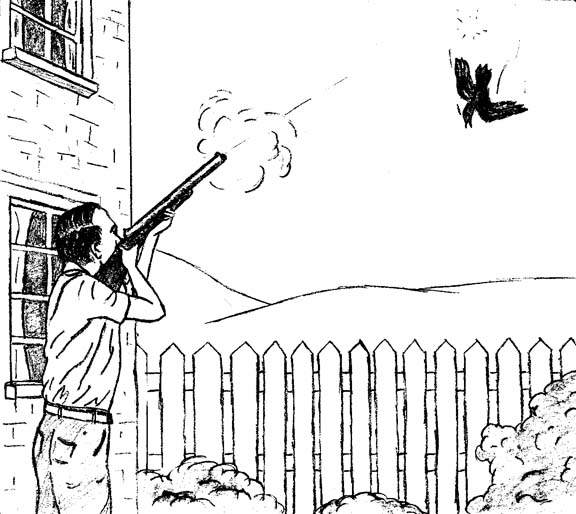
\includegraphics[width=.7\textwidth]{figures/exampleprompt2.jpg}
%\caption{This is an example figure from \citet{king:dickinson:13}.}
%\label{figure:KandD2013}
%\end{figure}
%
%\subsection{2014}
%\citet{king:dickinson:14}
%
%\subsection{2016}
%\citep{king:dickinson:16}
%
%\subsubsection{Bag-of-dependencies}
%Here we could discuss the switch to a bag-of-dependencies approach, the use of tf-idf and the use of vector cosine distance for ranking responses.
%
%\subsubsection{Clustering}
%Here we could briefly mention the clustering experiments we did in the 2016 paper. But really, I'd rather not, because I don't intend to repeat them in the dissertation.
%
%\subsection{2018}
%\cite{king:dickinson:18}
%
%\begin{figure}
%
\includegraphics[width=.7\textwidth]{figures/I29.jpg}
%\caption{This is an example figure from \citet{king:dickinson:18}.}
%\label{figure:KandD2018}
%\end{figure}


% This is a figure in landscape orientation
%\begin{sidewaysfigure}
%
\includegraphics[width=\textwidth]{figures/exampleFigure.png}
%\caption{This is another example Figure, rotated to landscape orientation.}
%\label{LandscapeFigure}
%\end{sidewaysfigure}

%While there is much current work on analyzing learner language, it
%usually focuses on grammatical error detection and correction
%\citep[e.g.,][]{HOO2012} and less on semantic analysis.  At the same
%time, Intelligent Computer-Assisted Language Learning (ICALL) and
%Intelligent Language Tutoring (ILT) systems
%\citep[e.g.,][]{heift:schulze:07, meurers:12} also tend to focus more
%on grammatical feedback. An exception to this rule is \textit{Herr
%  Komissar}, an ILT for German learners that includes rather robust
%content analysis and sentence generation \citep{desmedt:95}, but this
%involves a great deal of hand-built tools and does not connect to
%modern NLP.  Some work addresses content assessment for short answer
%tasks \citep{Meurers.Ziai.ea-11}, but this is still far from naturalistic,
%more conversational interactions \citep[though, see][]{petersen:10}.
%
%Our overarching goal is to facilitate ILTs and language assessment tools that maximize free
%interaction, building as much as possible from existing NLP resources.
%While that goal is in the distant future, the more immediate goal in
%this paper is to pinpoint the precise challenges which interactive
%learner sentences present to constructing semantic analyses, even when
%greatly constrained.  We approximate this by collecting data from a
%task which models some aspects of interaction, namely a picture
%description task (PDT), parsing it with an off-the-shelf parser,
%extracting semantic forms, and noting the challenges throughout.
%
%The focus towards interaction is in accord with contemporary theory
%and research in Second Language Acquisition (SLA) and best practices
%in second language instruction, which emphasize the limiting of
%explicit grammar instruction and feedback in favor of an approach that
%subtly integrates the teaching of form with conversation and
%task-based learning \citep{CelceMurcia:1991:GrammarPedagogy,
%  CelceMurcia:2002:GrammarThroughContext,
%  LarsenFreeman:1991:TeachingGrammar}.  Indeed,
%\citet{Ellis:2006:CurrentIssues} states, ``a traditional approach to
%teaching grammar based on explicit explanations and drill-like
%practice is unlikely to result in the acquisition of the implicit
%knowledge needed for fluent and accurate communication.''  For our
%purposes, this means shifting the primary task of an ICALL application
%from analyzing grammar to evaluating semantic appropriateness and
%accuracy.
%
%The data for error detection work is ideal for developing systems
%which provide feedback on essays, but not necessarily for more
%interactive communication.  Thus, our first step is to collect data
%similar to what we envision processing in something like an ILT game,
%data which---as far as we know---does not exist.  While we desire
%relatively free production, there are still constraints; for games,
%for example, this comes in the form of contextual knowledge (pictures,
%rules, previous interactions).  To get a handle on variability under a
%set of known constraints and to systematically monitor deviations from
%target meanings, we select a PDT as a constrained task that still
%promotes interactive communication.
%Collecting and analyzing this data is our first major contribution, as
%described in section~\ref{sec:data}.
%
%Once we have the data, we can begin to extract semantic forms, and our
%second major contribution is to outline successes and pitfalls in
%obtaining shallow semantic forms in interactive learner data, as
%described in section~\ref{sec:method}, working from existing tools.
%Although we observe a lot of grammatical variation, we will
%demonstrate in section~\ref{sec:evaluation} how careful selection of
%output representations (e.g., the treatment of prepositions) from an
%off-the-shelf parser and a handful of syntax-to-semantics rules allow
%us to derive accurate semantic forms for most types of transitive verb
%constructions in our data.  At the same time, we will discuss the
%difficulties in defining a true gold standard of meanings for such a
%task.  Finally, we examine methods for automatically correcting misspellings, showing that preprocessing with spelling correction tools and language modeling can significantly reduce downstream errors. This work paves the way for increasing the range of
%constructions and further exploring the space between free and
%constrained productions \citep[see also the discussion
%in][]{Amaral.Meurers-11}.

%\section{Related Work}
%
%In terms of our overarching goals of developing an interactive ILT,
%a number of systems exist (e.g., TAGARELA
%\citep{Amaral.Meurers.Ziai-11}, e-Tutor \citep{heift:01}), but few
%focus on matching semantic forms.  \textit{Herr Komissar}
%(\citet{desmedt:95}) is one counter-example; in this game, learners
%take on the role of a detective tasked with interviewing suspects and
%witnesses. The system relies largely on a custom-built database of
%verb classes and related lexical items. Likewise, \citet{petersen:10}
%designed a system to provide feedback on questions in English,
%extracting meanings from the Collins parser \citep{collins:99}.  Our
%work is is in the spirit of his, though our starting point is to
%collect data of the type of task we aim to analyze, thereby
%pinpointing how one should begin to build a system.
%
%The basic semantic analysis in this paper parallels work on content
%assessment (e.g., ETS's c-rater system
%\citep{leacock:chodorow:03}).  Different from our task, these systems
%are mostly focused on essay and short answer scoring, though many focus on semantic
%analysis under restricted conditions. As one example,
%\citet{Meurers.Ziai.ea-11} evaluate English language learners' short
%answers to reading comprehension questions, constrained by the topic
%at hand. Their approach performs multiple levels of annotation on the
%reading prompt, including dependency parsing and lexical analysis from
%WordNet \citep{Fellbaum:1998}, then attempts to align elements of the
%sentence with those of the (similarly annotated) reading prompt, the
%question, and target answers to determine whether a response is
%adequate or what it might be missing.  Our scenario is based on
%images, not text, but our future processing may need to
%include similar elements, e.g., determining lexical relations from
%WordNet.
%




%
%@article{alexopoulou2017task,
%  title={Task effects on linguistic complexity and accuracy: A large-scale learner corpus analysis employing natural language processing techniques},
%  author={Alexopoulou, Theodora and Michel, Marije and Murakami, Akira and Meurers, Detmar},
%  journal={Language Learning},
%  volume={67},
%  number={S1},
%  pages={180--208},
%  year={2017},
%  publisher={Wiley Online Library}
%}
%
%Justifying reliance on NLP tools to process NNS data:
%However, prior studies have shown that native language taggers and parsers perform fairly well on the learner data in EFCAMDAT (Geertzen et al., 2014). For example, Alexopoulou, Geertzen, Korhonen, and Meurers (2015) evaluated the accuracy of extraction of relative clauses, reporting an F score of 83.9%, and found that state-of-the-art NLP tools provide reasonable quality.
%
%#####
%
%
%
%
%@article{papadimitriou2021multilingual,
%  title={Multilingual BERT, Ergativity, and Grammatical Subjecthood},
%  author={Papadimitriou, Isabel and Chi, Ethan A and Futrell, Richard and Mahowald, Kyle},
%  journal={Proceedings of the Society for Computation in Linguistics},
%  volume={4},
%  number={1},
%  pages={425--426},
%  year={2021}
%}
%###
%
%@article{yamazaki2014,
%  title={Toward integrative CALL: A progressive outlook on the history, trends, and issues of CALL},
%  author={Yamazaki, Kasumi},
%  journal={TAPESTRY},
%  volume={6},
%  number={1},
%  pages={6},
%  year={2014}
%}
%"...sociocultural theories of learning, mainly named as Kolb�s (1984) experiential learning and Lave and Wenger�s (1991) situated learning, which emphasize that learning occurs in a communicative context through concrete and direct experiences. Learning in this approach is generally exploratory, thus learners� autonomy, engagement, and, most importantly, motivation are often found to be the most critical elements of contemporary CALL research (cf. Rahimi & Yodollahi, 2011; Ushioda, 2000; Schwienhorst, 2002; Mohammadi, Ghorbani, & Hamidi, 2011; AbuSeileek, 2012)."
%#####
%#####
%@article{collentine2011,
%  title={Learner autonomy in a task-based 3D world and production},
%  author={Collentine, Karina},
%  journal={Language Learning \& Technology},
%  volume={15},
%  number={3},
%  pages={50--67},
%  year={2011},
%  publisher={University of Hawaii National Foreign Language Resource Center}
%}
%With widespread access to technology, learners are increasingly using CALL materials in a learner- centered approach where they take control of their own learning, on their own time, and for their own purposes. These materials include virtual and 3D environments with gaming-like experiences (Darasawang & Reinders, 2010; Sykes, 2009). Highly interactive, multi-sensory environments provide access to real world simulations (Pantelidis, 1993; Schwienhorst, 2008), popularizing online multiuser virtual environments (e.g., Second Life) and massively multiplayer online games (e.g., World of Warcraft). In these autonomous learning environments entailing �independent action� and �decision- making� (Little, 1991, p. 4), it is essential that learners become cognizant of how to learn by raising their metalinguistic awareness and participating in tasks that motivate L2 communication. Fischer (2007) and Schwienhorst (2008) argue that learners in these environments should develop metacognitive abilities, strategies, and have opportunities for reflection (e.g., on input characteristics or their own learning strategies).
%#####
%#####
%@inproceedings{granstrom2004towards,
%  title={Towards a virtual language tutor},
%  author={Granstr{\"o}m, Bj{\"o}rn},
%  booktitle={InSTIL/ICALL Symposium 2004},
%  year={2004}
%}
%In learning a foreign language, visual signals may in many contexts be more important than verbal signals. During the process of acquiring a language, both child L1 speakers and adult L2 speakers rely on gestures to supplement their own speech production (McNeill, 1992; Gullberg, 1998). Adult L2 speakers often make more exten- sive use of gestures than L1 speakers, especially when searching for words or phrases in the new language. In this context, gestures have a compen- satory function in production, often substituting for an unknown word or phrase. L2 listeners may also make greater use of visual cues to aid the conversational flow than do L1 listeners. In this respect, parallels can be made between the situa- tion of the hearing impaired listener and the L2 learner (McAllister 1998).
%It has been found that the integration of seg- mental audio-visual information is affected by the relationship between the language of the speaker and that of the listener. Subjects listening to a for- eign language often incorporate visual informa- tion to a greater extent than do subjects listening to their own language (Kuhl et al. 1994; Burnham and Lau 1999). Furthermore, in a conversation, the L2 learner must not only concentrate on seg- mental phonological features of the target lan- guage while remembering newly learned lexical items, but must also respond to questions at the same time. This task creates a cognitive load for the L2 listener which is in many respects much different from that for the L1 user of a spoken dialogue system. Thus, the compensatory possi- bilities of modality transforms and enhancements of the visual modality are well worth exploring not only concerning segmental, phoneme-level information but also for prosodic and conversa- tional information.
%2 CALL-related projects at CTT
%The CALL research at the Centre for Speech Technology (CTT) focuses on building a Virtual Language Tutor, using an animated talking agent, that addresses these issues, serving as a conversa- tional partner, teacher and an untiring model of pronunciation, who can pick exercises from a training library depending on the user�s needs.
%#####
%#####
%@article{heift2001intelligent,
%  title={Intelligent language tutoring systems for grammar practice},
%  author={Heift, Trude},
%  journal={Zeitschrift f{\"u}r Interkulturellen Fremdsprachenunterricht},
%  volume={6},
%  number={2},
%  year={2001}
%}
%The present paper discusses building a more flexible Web-based grammar practice environment around an Intelligent Language Tutoring System (ILTS). While ILTSs employ Natural Language Processing (NLP) and thus require programming and linguistic expertise, they provide error-specific feedback and flexibility in handling student answers. Sound, graphics and/or videos can also be implemented to achieve a more varied, authentic and contextualized learning environment.
%#####
%#####
%@article{nagata:02,
%	Author = {Noriko Nagata},
%	Date-Added = {2010-08-12 15:04:17 -0400},
%	Date-Modified = {2010-10-19 12:57:46 -0400},
%	Journal = {{CALICO} Journal},
%	Key = {system},
%	Keywords = {ICALL, Japanese},
%	Note = {\url{http://www.usfca.edu/japanese/CALICO02.pdf}},
%	Number = 3,
%	Pages = {583-599},
%	Title = {{BANZAI}: An Application of Natural Language Processing to Web based Language Learning},
%	Volume = 19,
%	Year = 2002}
%
%The BANZAI program, however, is written in Java, which pro- vides excellent support both for sophisticated NLP programming and ap- pealing multimedia applications. As a result, the BANZAI interface is user friendly and visually appealing, making full use of digital photographs, computer graphics, pull down menus, button selections, and Japanese sounds. Each exercise in BANZAI is framed in a conversational setting, along with a relevant photographic or graphical image of Japan, and asks learners to produce a target sentence that is likely to be uttered in real communicative situations.


